% ****** Start of file aipsamp.tex ******
%
%   This file is part of the AIP files in the AIP distribution for REVTeX 4.
%   Version 4.1 of REVTeX, October 2009
%
%   Copyright (c) 2009 American Institute of Physics.
%
%   See the AIP README file for restrictions and more information.
%
% TeX'ing this file requires that you have AMS-LaTeX 2.0 installed
% as well as the rest of the prerequisites for REVTeX 4.1
%
% It also requires runnin. The commands are as follows:
%
%  1)  latex  aipsamp
%  2)  bibtex aipsamp
%  3)  latex  aipsamp
%  4)  latex  aipsamp
%
% Use this file as a source of example code for your aip document.
% Use the file aiptemplate.tex as a template for your document.
\documentclass[%
 aip,
%jmp,%
%bmf,%
rsi,
 amsmath,amssymb,
%preprint,%
 reprint,%
%author-year,%
%author-numerical,%
]{revtex4-1}

\usepackage{graphicx}% Include figure files
\usepackage{dcolumn}% Align table columns on decimal point
\usepackage{bm}% bold math
\usepackage{url}
%\usepackage[mathlines]{lineno}% Enable numbering of text and display math
%\linenumbers\relax % Commence numbering lines

\begin{document}

\preprint{AIP/123-QED}

\title{The NeXus Data Format}


\author{Mark K\"onnecke}
\affiliation{Laboratory for Development and Methods, Paul Scherrer Institute, 5232 Villigen-PSI, Switzerland}

\author{Frederick Akeroyd}
\affiliation{ISIS, Rutherford Appleton Laboratory, UK}

\author{Herbert J Bernstein}
\affiliation{imgCIF, Dowling College, USA}

\author{Aaron S. Brewster}
\affiliation{Lawrence Berkeley National Laboratory, USA}

\author{Bjoern Clausen}
\affiliation{Los Alamos National Laboratory, USA}

\author{Stephen Cottrell}
\affiliation{ISIS, Rutherford Appleton Laboratory, UK}

\author{Jens Uwe Hoffmann}
\affiliation{Helmholtz Zentrum Berlin, Germany}

\author{Pete R. Jemian}
\affiliation{Advanced Photon Source, Argonne National Laboratory, USA}

\author{David M\"annicke}
\affiliation{ANSTO, Australia}

\author{Raymond Osborn}
\affiliation{Argonne National Laboratory, USA}

\author{Peter F. Peterson}
\affiliation{Spallation Neutron Source, USA}

\author{Tobias Richter}
\affiliation{Diamond Light Source, UK}

\author{Jiro Suzuki}
\affiliation{KEK, Japan}

\author{Benjamin Watts}
\affiliation{Swiss Light Source, Paul Scherrer Institute, 5232 Villigen-PSI, Switzerland}

\author{Eugen Wintersberger}
\affiliation{Deutsches Elektronen-Synchrotron DESY,D-22607 Hamburg,Germany}

\author{Joachim Wuttke}
\affiliation{Forschungszentrum J\"ulich, JCNS at MLZ, Garching, Germany}


\collaboration{NeXus International Advisory Committee}

\date{\today}% It is always \today, today,
             %  but any date may be explicitly specified

\begin{abstract}
NeXus is an effort by an international group of scientists to define 
 a common data exchange format for neutron, X-ray, and muon experiments.   
NeXus is built on top of the scientific data format HDF5 and adds 
domain-specific 
rules for organizing data within HDF5 files in addition to a dictionary of well-defined 
domain-specific field names. The NeXus data format has two purposes.  First, NeXus defines a
format that can serve as a container for all relevant data associated
with a beamline. This is a very important use case.  Second, NeXus
defines standards in the form of \emph{application definitions} for the
exchange of data between applications.  NeXus provides structures for raw experimental data as well as for processed data.  
\end{abstract}

%%\pacs{Valid PACS appear here}% PACS, the Physics and Astronomy
                             % Classification Scheme.
\keywords{NeXus, data format, HDF5, X-ray, neutron, data analysis, data management}
\maketitle


\section{Introduction}
Increasingly, major neutron and X-ray facilities have chosen to store their data in the NeXus data format. 
Since 2006, NeXus\cite{nxold} has undergone substantial refocusing, 
refinement and enhancement as described in this paper.  

Historically, neutron and X-ray facilities choose to store their data in a plethora of 
home-grown data formats. This scheme has a number of drawbacks addressed by NeXus: 
\begin{itemize}
\item It makes the life of traveling scientists unnecessarily difficult as they have to deal with multiple files 
 in different formats, file converters and such in order to extract scientific information from the data.
 \item An unnecessary burden is imposed on data analysis software producers as they have to accommodate so many different formats.  
\item The whole idea of open access to data is sabotaged if the data is in a format which cannot be easily understood.
\item Scientific integrity is jeopardized if the data cannot be understood. Or important elements are missing.
\item Modern high speed detectors produce data at such a high rate that many older single image storage schemes 
 have become impractical and 
 an efficient container format is a necessity. 
\end{itemize}

The first necessity for a data format is a physical file format: how is the data written to disk? Rather than inventing  
yet another format, NeXus chose HDF5\cite{hdf5} as the binary container format. HDF5 is efficient, self-describing, 
platform-independent, in the public domain and well supported by both commercial and free software tools. 

NeXus adds to HDF5:
\begin{itemize}
\item Rules for organizing domain-specific data within a HDF5 file
\item A link structure to enable quick default visualization
\item A dictionary of documented domain-specific field names
\item Definitions of standards that can be validated
\end{itemize}

The development of NeXus is overseen by a committee, the NeXus International Advisory Committee (NIAC).

\section{NeXus Design Principles}

The authors of data-acquisition and instrument-control software are encouraged to generate exactly \emph{one} NeXus container file per measurement
(a measurement is either a data accumulation under fixed conditions,
or a scan).
This file includes not only the detector and monitor data,
but also metadata, information on the state of the beamline, parameter logs, and more.
Authors of data-reduction and data-analysis software can use NeXus to
store processed data along with metadata and a processing log.

NeXus data files are built using basic HDF5 storage elements: 
data groups (like file system folders), 
data fields (such as strings, floats, integers, and arrays), 
attributes (additional descriptors of groups and fields), 
and links (like file system links).  These basic storage elements are used to
build the \emph{base classes}, \emph{application definitions},
and \emph{contributed definitions} that elaborate the NeXus standard.

As a container format, NeXus allows files to be extended at any moment by
additional entries.
A special base class, \texttt{NXcollection}, exempts its contents from validation
and thereby allows inclusion of whatever data in arbitrary non-NeXus formats.

NeXus can be used for many different experimental techniques,
and at different levels of data processing.
For each of these different applications,
a specific subset of the standardized NeXus entities 
(data groups and fields) is needed.
These subsets, and their hierarchical structure, are standardized
in the NeXus application definitions (Sect.~\ref{sect_appdef}).

\section{NeXus File Hierarchies}
NeXus data files are organized into a hierarchy of groups which, in turn, can contain further groups or fields, 
very much like an internal file system. The content of each NeXus group is defined by either a base class, 
an application definition, or a contributed definition.


\subsection{NeXus Raw Data File Hierarchy}
For an overview of the NeXus data file structure for raw experimental data see FIG.~\ref{rawfile}.
\begin{figure}
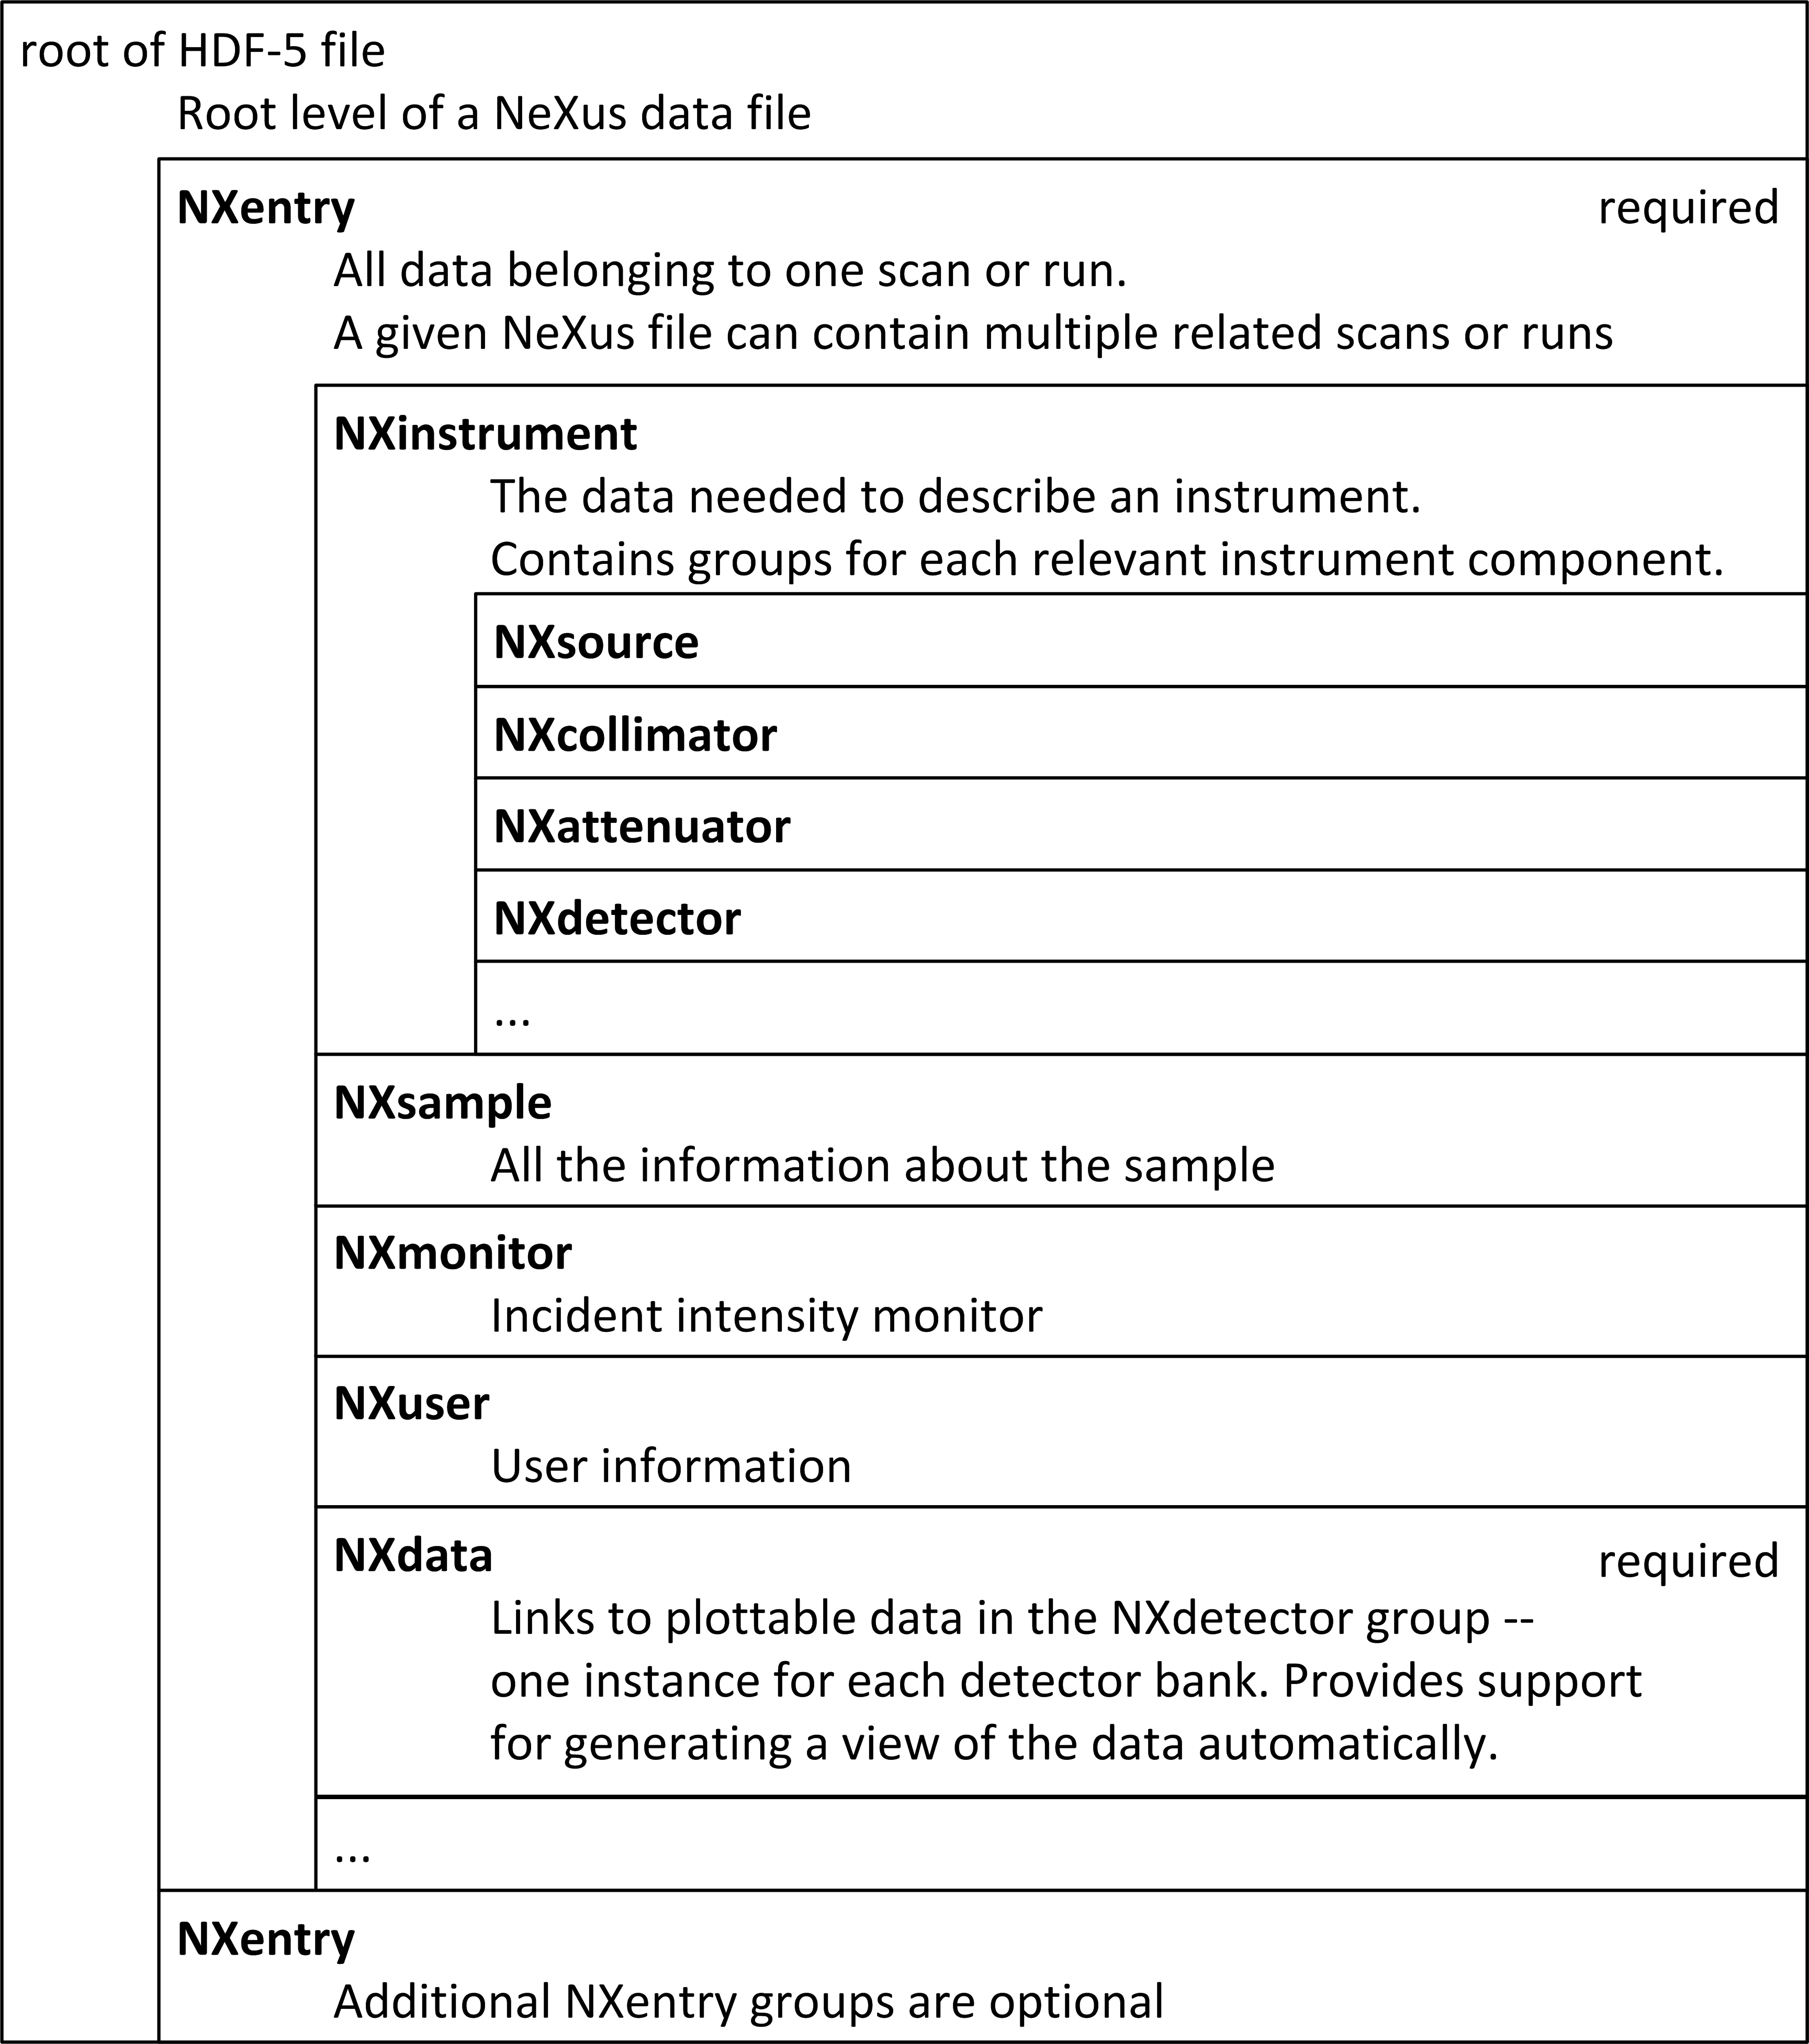
\includegraphics[width=\columnwidth]{figure1}
\caption{\label{rawfile}Overview of the structure of a NeXus raw data file.}
\end{figure}

The major focus of NeXus has been the recording of ``raw'' experimental data, i.e. information taken directly from the experimental 
equipment, or processed only as required to provide physically meaningful values.
The NeXus raw data file hierarchy is the consequence of some practical considerations. When looking at a beamline it is easy to 
discern different components: beam optic components, sample position, detectors and such. It is quite natural to mirror this physical 
separation with a logical arrangement of storing the data from each component in a separate group. This approach explains the 
list of beamline components in the \texttt{NXinstrument} group presented in FIG.~\ref{rawfile}. 
As there can be multiple instances of the same kind of equipment, like slits or detectors, in a given beamline it becomes necessary
to add type information to the group name. This type information is provided by a HDF5 attribute, the NeXus class name.
By convention NeXus class names start 
with the prefix \texttt{NX}. Each NeXus group describing a beamline component contains further groups and fields describing the component. 
A field can contain a single number, a text string or an array, as appropriate to the data to be described.  

The requirement to store multiple related scans or runs  in the same file or to capture 
a complete workflow in a file causes the beamline component hierarchy to be pushed one level deeper into an \texttt{NXentry} 
group in the hierarchy. The \texttt{NXentry}  group thus represents one scan or run (or a processed data entry, as will be discussed later). 
The \texttt{NXentry} group also holds the experiment metadata, such as the date and time at which it was performed. 

In the course of NeXus history,
the decision was taken to move \texttt{NXmonitor}
out of \texttt{NXinstrument} to the higher hierarchy level of \texttt{NXentry},
in order to facilitate quick inspection by humans.

To enable a simple default visualization,
a \texttt{NXdata} group must be provided at \texttt{NXentry} level.
It contains information about plot axes and links to the data
(which typically reside in the \texttt{NXdetector} group).
Links are supported by HDF5 and work like symbolic links in the Unix file system.

\subsubsection{Multiple Method Instruments}

Particularly at X-ray sources,
some instruments offer multiple techniques that can be used in parallel.
For example small-angle scattering and powder diffraction 
can be measured simultaneously at a SAXS/WAXS beamline.
We recommend storing the results from all subinstruments in \emph{one} file.
All data are stored in one and the same \texttt{NXentry} hierarchy
(FIG.~\ref{multimethod}). All information from all detectors, logs and 
such are collected in one \texttt{NXentry} to keep the data together.
Information that is peculiar for one experimental technique
is linked  into a \texttt{NXsubentry}. The NXsubentry follows the hierarchy of 
\texttt{NXentry}. But it will typically only links to the data required by the 
application definition for the specific experimental technique. The point of this scheme 
is that human and computerized users can easily locate method specific data. But thereby 
maintaing the full view of the experiment.   

\begin{figure}
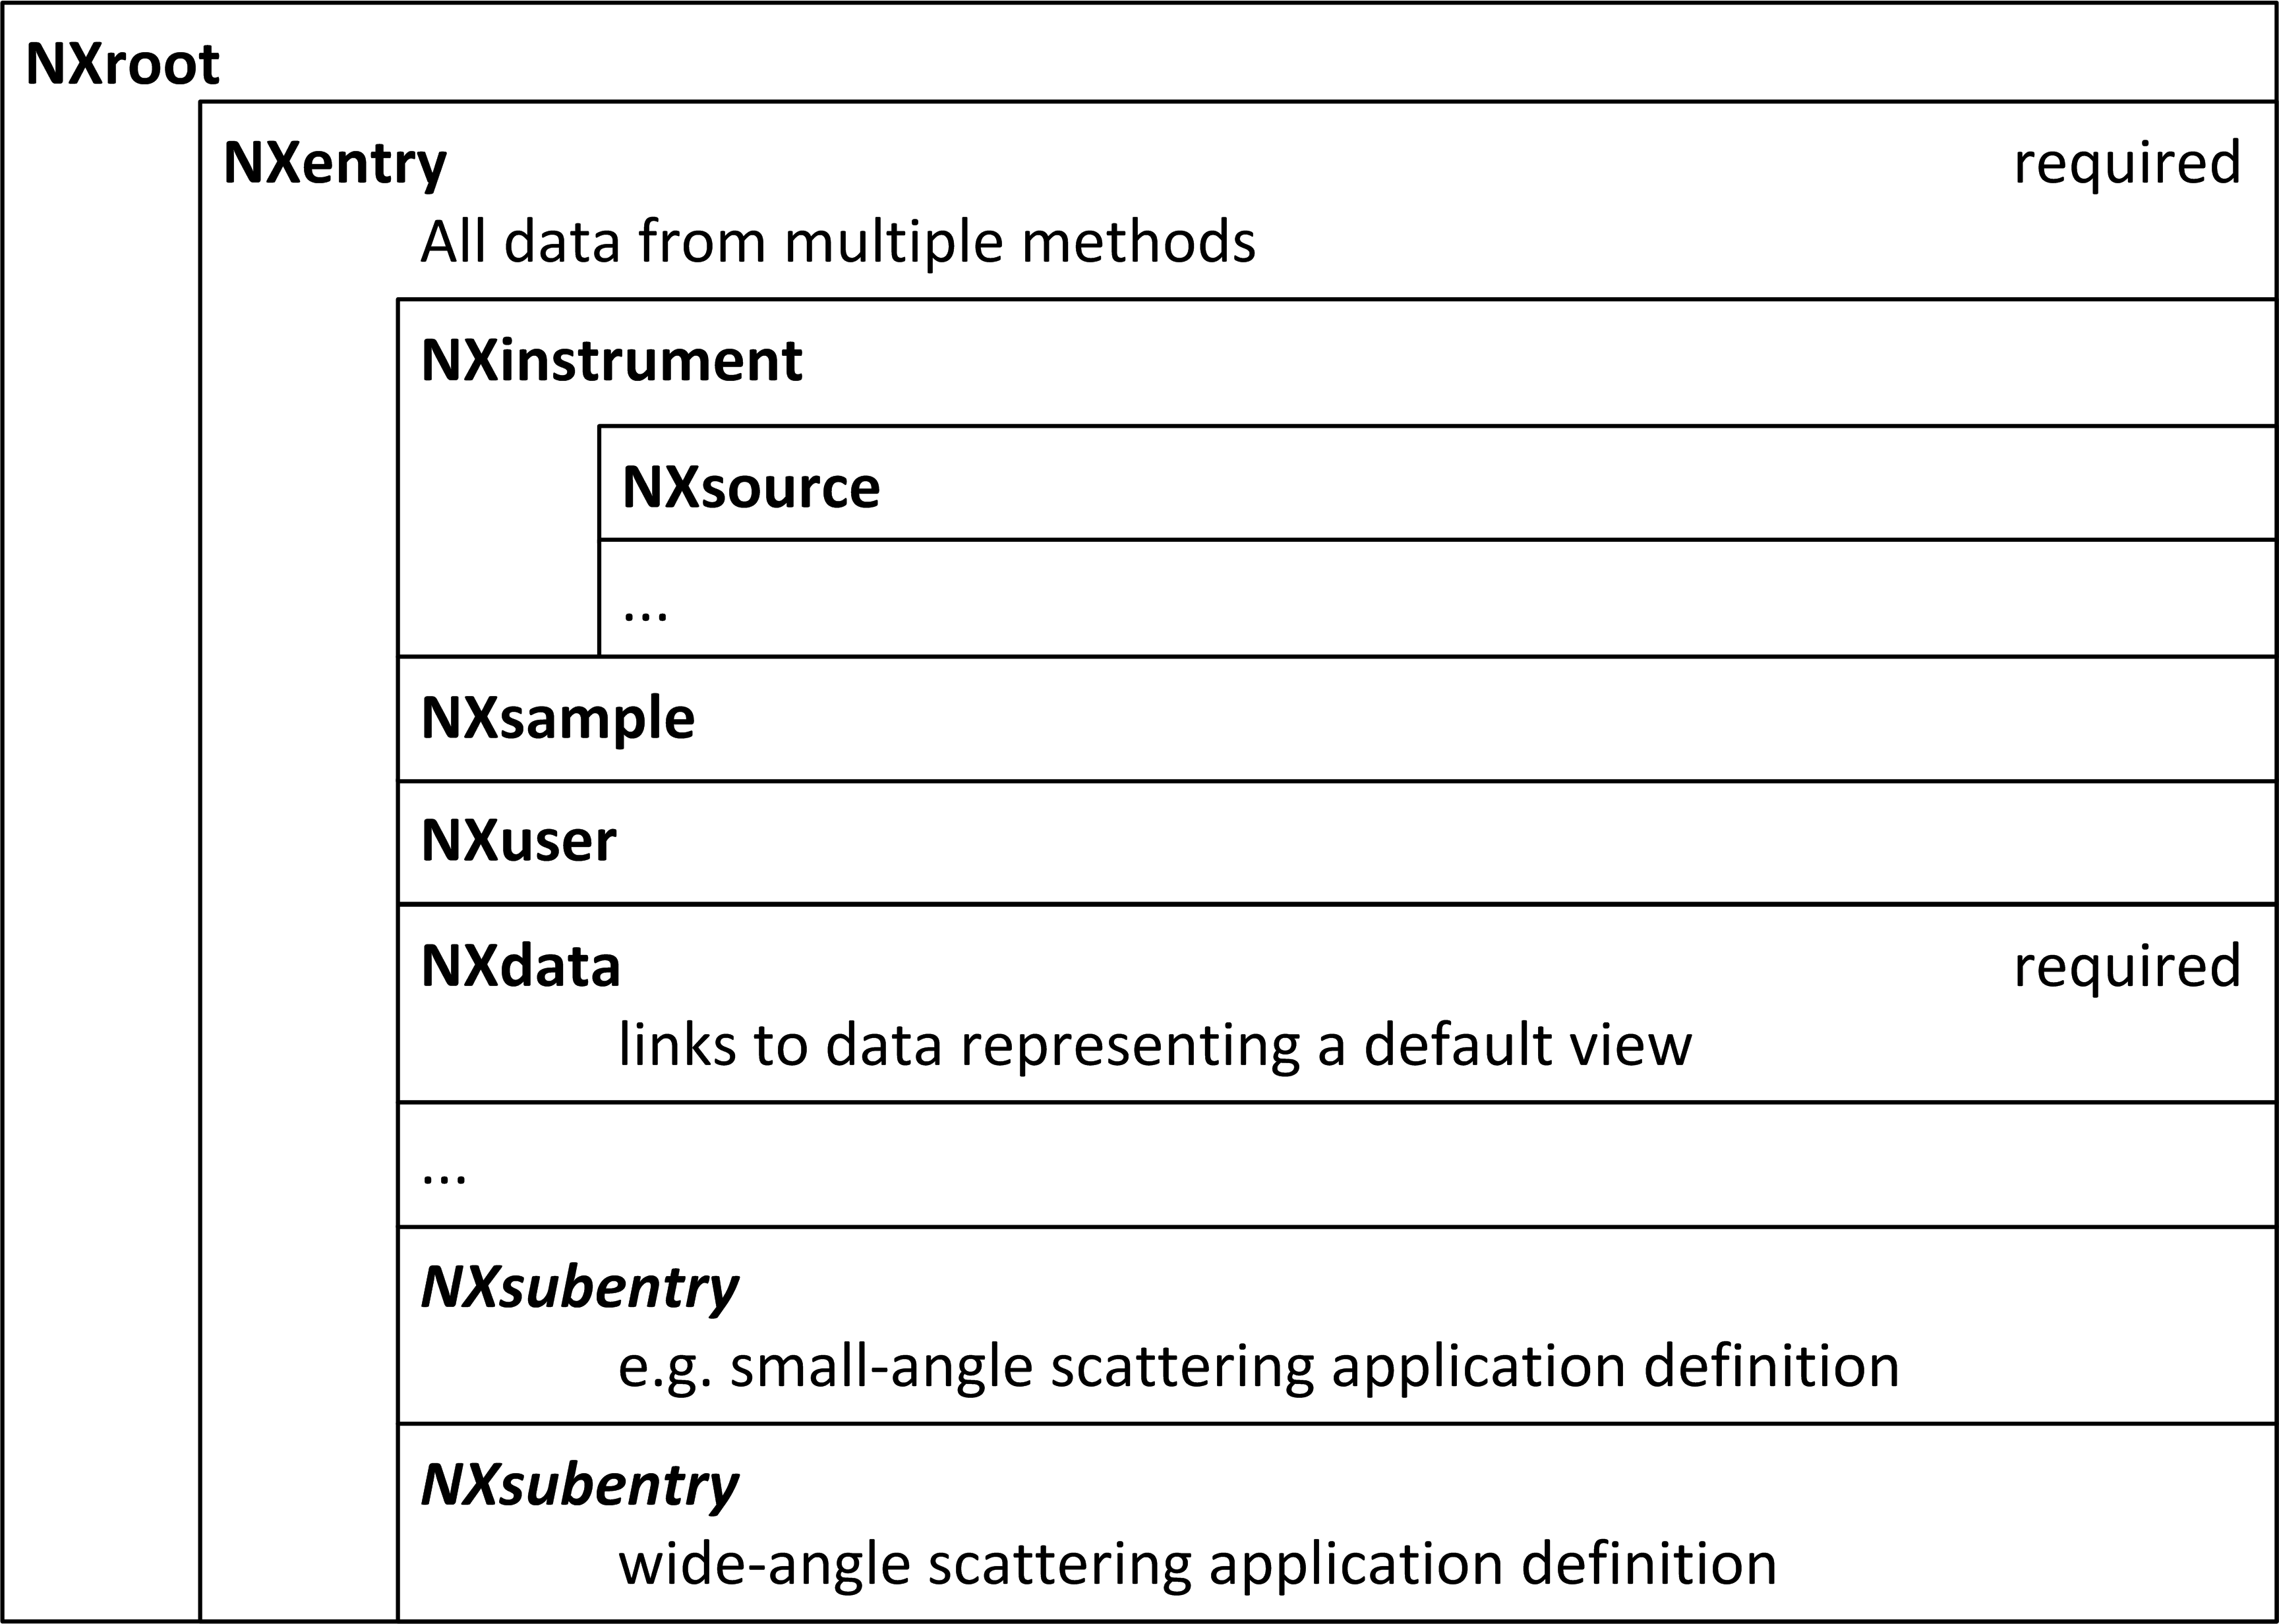
\includegraphics[width=\columnwidth]{figure2}
\caption{\label{multimethod}Overview of the structure of a NeXus raw data file for an instrument with multiple methods.}
\end{figure}

\subsubsection{Scans}

Scans come in all shapes and sizes. Almost anything can be scanned against anything. 
An additional difficulty is that, in practice, the number of scan points in the scan 
cannot be known in advance since it is possible that a scan may be interrupted or terminated
before its planned number of observations. 
Thus, it is a challenge to standardize a scan.
NeXus solves these difficulties through 
a couple of conventions and the use of a HDF5 feature called unlimited dimensions. With the HDF5 
unlimited dimensions feature, one axis of the data is allowed to expand without limit and 
the size of a data array does not need to be declared in advance. Data can be appended 
to an array along the unlimited dimension as required. 

Scans are stored in NeXus following these conventions: 
\begin{itemize}
\item Each variable varied or collected in the scan is stored at its appropriate place in the NeXus beamline 
 hierarchy as an array. The array's first dimension is the scan axis. This is the unlimited dimension in 
 the implementation and data is appended at each scan point to the array. 
\item The \texttt{NXdata} group holds links to all the variables varied or collected during the scan. 
 This creates something equivalent to or better than the tabular representation people are used to for scans. 
 The main detector data can be plotted against any scanned parameter as well as against everything that was 
 deemed worth recording in addition to that.  The necessary data is all gathered together in the \texttt{NXdata}
 group either directly or via links, so that other groups do not
 normally have to be searched to do this plotting.
 
\end{itemize}

NeXus allows multi-dimensional scans too. This makes it very simple to produce meaningful slices through data 
volumes even with NeXus-agnostic software (like hdfview). Interrupting a multi-dimensional scan may, depending 
on the software used, leave some of the data in an uninitialised state (usually the HDF5 fill value).



\subsection{Processed Data}

At the request of the user community, NeXus created a simplified structure for storing the result of data 
processing: be it reduction or analysis. In many cases even the reduced data is big enough to need 
an efficient binary representation. A good example is a tomography reconstruction. A tabular representation 
of the NeXus processed data file structure is given in FIG.~\ref{procfile}. 

\begin{figure}
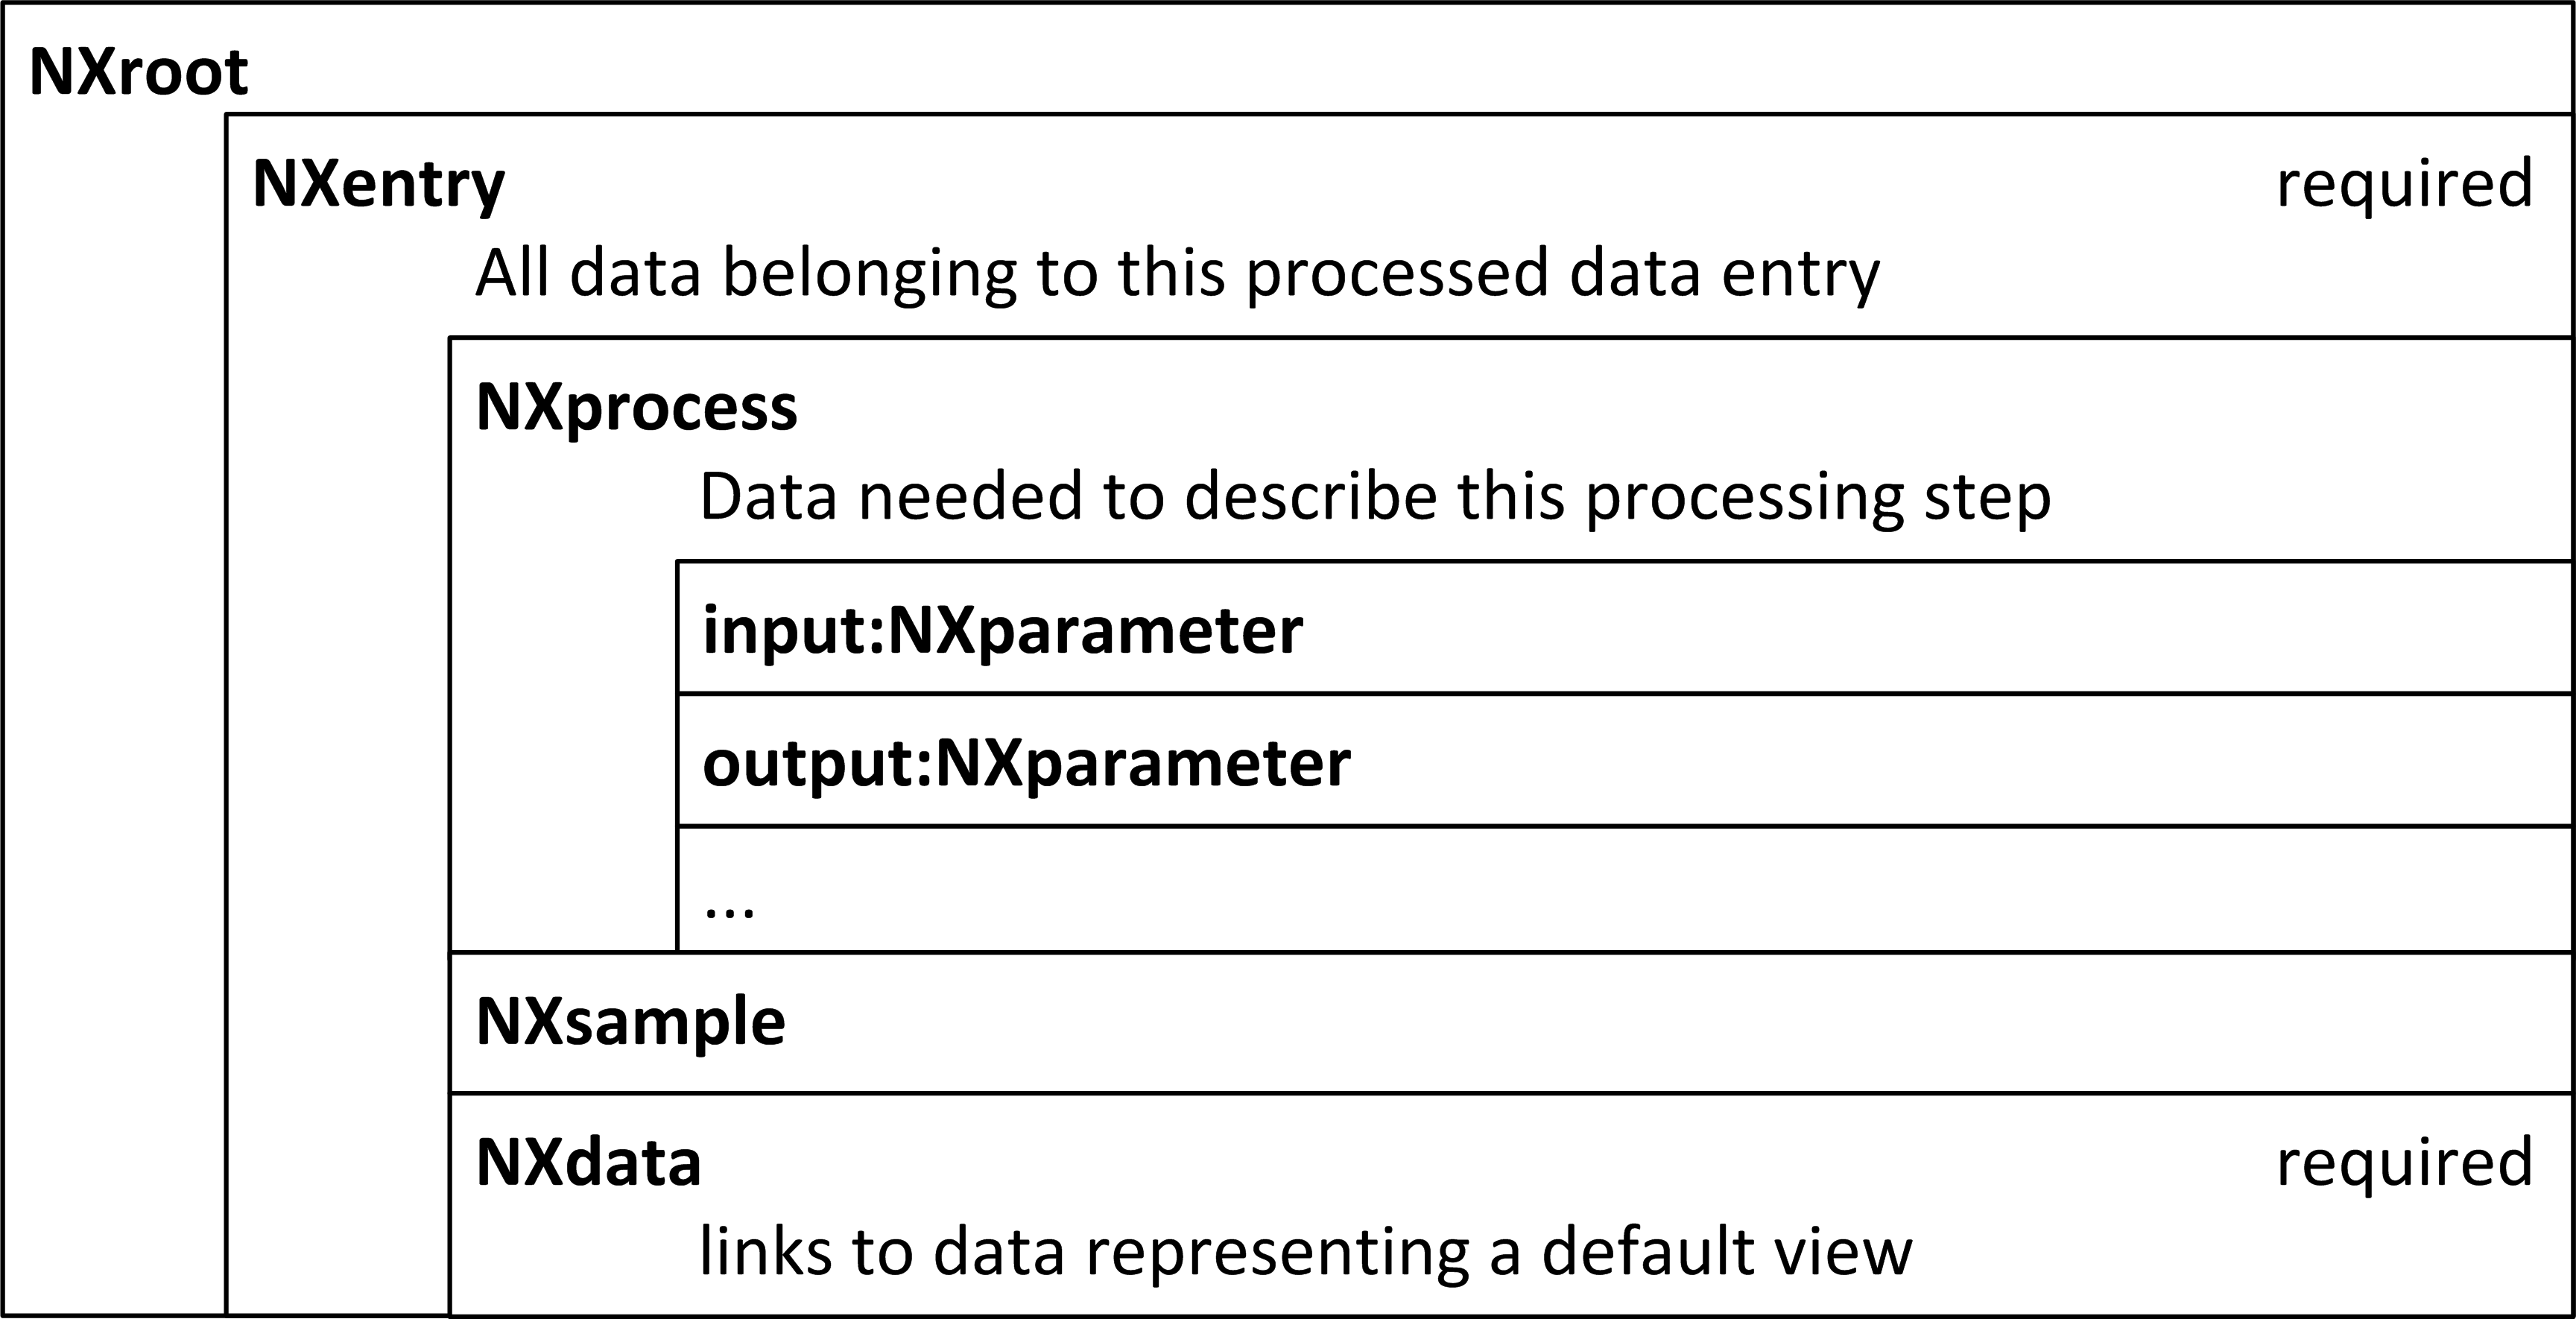
\includegraphics[width=\columnwidth]{figure3}
\caption{\label{procfile}Overview of the structure of a NeXus processed data file.}
\end{figure}

The hierarchy is much reduced as it is not important to carry all experimental information in the data 
reduction. In contrast to the raw data file structure, \texttt{NXdata} in the processed file structure is the place 
to store the results of the processing, together with its associated axes if the result is a multi-dimensional array.   
 
Information about the sample and instrument can be stored in \texttt{NXsample} and \texttt{NXinstrument} groups as required. 

In addition, there is a new structure to store details about the processing such as the program used, its version, 
the date of processing, and other metadata 
in the \texttt{NXprocess} group. The \texttt{NXprocess} group can hold additional \texttt{NXparameter} groups which are containers 
for storing the input and output parameters of the program used to perform the processing. 

\section{Coordinate Systems, Positioning of Components and Further Rules}

For analysing data it is often necessary to know the exact position and orientation of beamline components. 
The first thing needed is a reference coordinate system. NeXus chose to use same coordinate system as the 
neutron beamline simulation software McStas\cite{mcstas}. 

For describing the placement and orientation of components, NeXus stores the same information as used for the 
same purpose in the Crystallographic Interchange Format (CIF)\cite{ITCVG}. CIF (and NeXus) stores the details 
of the translations and rotations necessary to move a given component from the zero point of the coordinate 
system to its actual position. As coordinate transformations are not commutative, the order of transformations 
must also be stored.

Many fine details of the NeXus format have been thoroughly discussed and are now well defined, but for the sake 
of brevity, we will not present an exhaustive view of NeXus here. A full listing of NeXus rules is given in the 
NeXus manual\cite{nxman}. Some examples of these additional rules include those governing:
\begin{itemize}
\item How axes are associated with data
\item That units must be given with the data
\item How data is to be stored in NeXus fields
\item How to describe array data which is not in ANSI C storage order
\end{itemize}


\section{NeXus Base Classes}

As can be seen from the discussion of the NeXus file hierarchy, NeXus arranges data into groups which have a 
type descriptor, a NeXus base class name, associated with them.
Technically, the class name is the value of the HDF5 attribute \texttt{NXclass}.
The term \emph{base class} is not used in the same sense as in  
object-oriented programming languages; in particular, there is no inheritance.
A NeXus base class is rather a dictionary of allowed keywords.
These keywords designate data fields that can be stored within a group.
A data field can have a simple type (like integer, float, date/time, binary),
or it can be a NeXus subgroup.
The base class definition also contains informal annotations
about the semantics of each field.

At base class level, NeXus has no mechanism to mark some fields as obligatory.
All allowed fields are optional.
Which of them are written into data files must be decided
according to application needs.
These decisions can be standardized in form of
application definitions (see below, Sect.~\ref{sect_appdef}).

The NeXus base classes are encoded in NeXus Description Language (NXDL)\cite{nxman}. NXDL is 
just another application of XML. Thus a NXDL file is an XML file that specifies the content 
of the NeXus base classes. 


\section{NeXus Application Definitions}
  \label{sect_appdef}

An application definition specifies a data structure
for a given application domain.
The data structure consists of a hierarchy of NeXus groups.
For each group, a \emph{minimum} content is specified.
Application definitions are therefore complementary
to base class definitions, which specify the \emph{maximum} content of groups.

Typically, an application definition addresses one type of instrument,
like X-ray reflectometer,
or direct-geometry neutron time-of-flight spectrometer.
Therefore application definitions were originally named \emph{instrument definitions}.
However, as NeXus can also be used for processed data
like a tomography reconstruction or a dynamic scattering law $S(Q,\omega)$, 
the more generic term \emph{application definition} is preferred.

NeXus application definitions are expressed in NXDL.  They may be parsed either by humans or by software and 
they may be validated for syntax and content.  The NXDL files are used to validate the structure of
NeXus data files. A tool exists to perform such validation.%
% TODO: can we please add some kind of reference to where the validation tool can be found?
% JAVA source code is here:
% https://github.com/nexusformat/code/tree/master/applications/NXvalidate
% is there a JAR file available?

The process of drafting and ratifying application definitions
is ongoing (see also below, Sect.~\ref{sect_gov}).
Currently, scientists representing both
the NeXus International Advisory Committee and the IUCr Committee on the Maintenance
of the CIF standard 
are nearly finished with a NeXus application definition for macromolecular crystallography.
CBFlib\cite{cbflib} is being extended to work with NeXus-MX format. This work will be published in another paper. 
Work on another NeXus application definition for reduced small-angle scattering data
is also in progress\cite{cansas}  by scientists representing
canSAS, NeXus, and the IUCr Commission on Small-Angle Scattering.


\section{Uptake of NeXus} 

NeXus is already in use as the main data format at facilities like Soleil, Diamond, SINQ, SNS, Lujan/LANL 
and KEK. Other facilities like ISIS, DESY and the $\mu$SR community are in the process of moving towards 
NeXus as their data format. At LBNL, NeXus is currently being adapted for XFEL serial crystallographic data. 


The adoption of NeXus took time. The reason is that NeXus is often chosen whenever 
a facility starts operation or undergoes major refurbishments. For those facilities where there is an existing and working 
pipeline from data acquisition to data analysis,  the resources are usually lacking to move 
towards NeXus.

This is reflected in the experience of the muon community. For the ISIS source, the move to a Windows PC-based data acquisition 
system in 2002 required a new data format, providing an ideal opportunity to exploit the emerging NeXus standard\cite{muon1}. In 
contrast, sources at PSI, TRIUMF and KEK continued to make good use of existing formats and software. More recently, funding 
from the EU has enabled the community to develop the Application Definition as a common exchange format for muon data\cite{muon2}. 
Whether used as the main or an intermediate format, users will soon be able to produce compatible NeXus files for data written 
across all facilities, enhancing the uptake of NeXus within the community.


\section{NeXus Governance}
  \label{sect_gov}

The development of NeXus is overseen
by the NeXus International Advisory Committee (NIAC).
The NIAC seek balanced representation of the international community.
Most major neutron, X-ray, and muon facilities have already appointed delegates.
Other facilities are invited to join.

The NIAC reviews proposed amendments to the NeXus base classes and
application definitions, and holds online votes to ratify changes.
A great number of candidate NeXus application definitions exist which were derived from our understanding of the technique described.
For each of these, the NeXus team seeks community approval. 


\section{Backwards Compatibility}

Historically, NeXus supported reading and writing data files in HDF4, HDF5 and
XML formats by use of the NeXus Application Programming Interface
(NeXus-API or NAPI).  The NAPI is still available, but frozen except for bug fixes.
After consultation with the community the currently recommended use of
NeXus is solely in terms of the HDF5 file format, using standard HDF5 tools.
That is expected to remain the basis for NeXus software development and
file creation in the future.

\section{Summary}

NeXus has matured considerably over the last ten years and is now in use in many facilities. NeXus 
is flexible enough to accommodate a wide variety of instruments and scientific applications. 
Yet it is efficient enough to 
handle the data coming from modern high speed detectors.
More information, including a full PDF manual, can be found on
the project web site.\cite{nxwww}
Also, do not hesitate to contact members of the NIAC.


\nocite{*}
\bibliography{nexus14aip}% Produces the bibliography via BibTeX.

\end{document}
%
% ****** End of file aipsamp.tex ******
